%%%%%%%%%%%%%%%%%%%%%%%%%%%%%%%%%%%%%%%%%%%%%%%%%%%%%%%%%%%%%%%%%%%%%%%%%%%%%%%
% intro.tex: Introduction to the thesis
%%%%%%%%%%%%%%%%%%%%%%%%%%%%%%%%%%%%%%%%%%%%%%%%%%%%%%%%%%%%%%%%%%%%%%%%%%%%%%%%
\chapter{verification of models}
\label{verifi_chapter}
%%%%%%%%%%%%%%%%%%%%%%%%%%%%%%%%%%%%%%%%%%%%%%%%%%%%%%%%%%%%%%%%%%%%%%%%%%%%%%%%

\section{Validation and verification of the VLE solvers and CFD solver} \label{App:vali}


    \subsection{Validation of the TPn flash solver based on phase boundaries}
    The TPn flash solver is validated by comparing the predictions with the experimental data of Somait and Kidnay~\cite{somait1978liquid} in terms of the phase boundaries of \ce{CO2}/\ce{CH4} and \ce{CO2}/\ce{H2O} mixtures. As shown in Fig.~\ref{v1}, the model prediction agrees with the experimental data very well for both mixtures.
    \begin{figure}[htbp]
        \centering
        \subfigure{
            %\begin{minipage}[t]{0.5\linewidth}
            \centering
            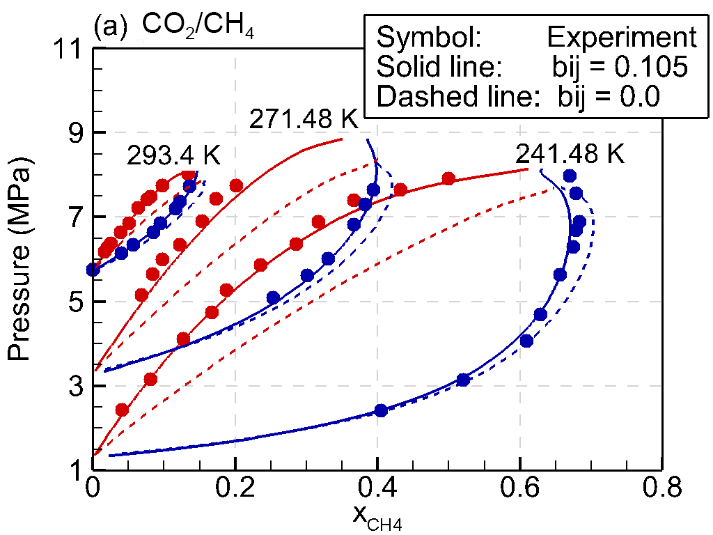
\includegraphics[width=0.45\linewidth]{phase_diagram_PX_CO2_CH4.png}
            %\caption{fig1}
            %\end{minipage}%
        }%
        \subfigure{
            %\begin{minipage}[t]{0.5\linewidth}
            \centering
            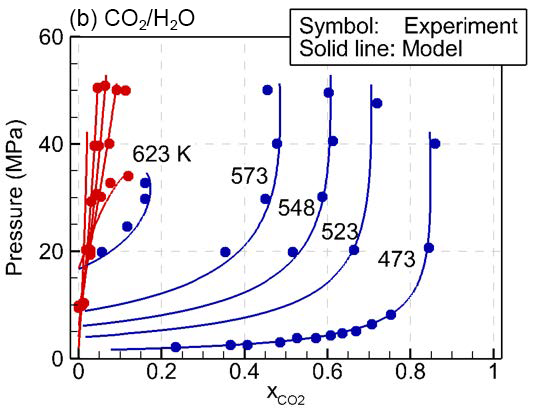
\includegraphics[width=0.45\linewidth]{phase_diagram_PX_CO2_H2O.png}
            %\caption{fig2}
            %\end{minipage}%
        }%
        \caption{Comparison of pressure-composition phase boundaries between experimental measurements and model predictions: (a) mixtures of \ce{CO2} and \ce{CH4}; (b) mixtures of \ce{CO2} and \ce{H2O}. Symbol: experimental data \citep{somait1978liquid}; line: model prediction. In sub-figure (a), solid line: binary interaction parameter $b_{ij}=0.105$ is used in Eqs.~(6-7) of the Supplementary Material; dashed line: $b_{ij}=0$ is used in Eqs.~(6-7) of the Supplementary Material. Red color: bubble points/curve, blue color: dew points/curve.}
        \label{v1}
    \end{figure}

    \subsection{Verification of the TPn flash solver based on mixture critical points}
    Next, the mixture critical points obtained from the VLE method (specifically, the TPn flash solver) are compared with those obtained from several other methods. In the VLE-based method, critical points can be obtained directly from the intersection of the dew curve and bubble curve.

    Stradi et al.~\cite{stradi2001reliable} derived the mixture critical point based on Heidemann and Khalil's criticality formulation~\cite{heidemann1980calculation} as below, which has been widely used due to its clear theoretical foundation. For a mixture of $C$ components,
    \begin{align}
         & Q\Delta \mathbf n=\mathbf0                                                                          \\
         & Q_{ij}=\left( \frac{\partial^2A}{\partial n_i \partial n_j}\right)_{T,V}                            \\
         & \sum_i^{C}\sum_{j}^{C}\sum_{k}^{C}A_{ijk}\Delta n_i\Delta n_{j}\Delta n_{k}=0                       \\
         & \Delta \mathbf n^{T}\Delta \mathbf n=1                                                              \\
         & A_{ijk}=\left( \frac{\partial^3A}{\partial n_i \partial n_j\partial n_k}\right)_{T,V} \label{eq:19}
    \end{align}
    where $\Delta \mathbf n$ means the nonzero perturbation vector of the component mole numbers; $A$ is the Helmholtz free energy. Since the Helmholtz free energy depends on the mixture composition, this way is implicitly dependent on the local mixture. The binary critical points predicted by the above methods are compared in Fig.~\ref{v2}, and the predictions of the current VLE-based method agree very well with Stradi et al.'s formulation~\cite{stradi2001reliable} for the mixture of \ce{CH4} and \ce{H2S}. But note that Stradi et al.'s formulation can only predict critical points, and it cannot provide other detailed information (e.g., phase boundaries) about phase diagrams like what VLE solver can provide.


    \begin{figure}[htbp]
        \begin{center}
            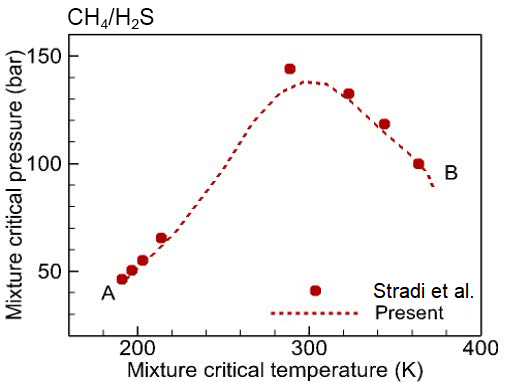
\includegraphics[width=0.55\linewidth]{critical_point_CH4_H2S.png}
            %\includegraphics[width=0.45\linewidth]{thermal/vali2_v2.png}
        \end{center}
        \caption{Comparison of predicted mixture critical points of \ce{CH4}/\ce{H2S} mixtures between Stradi et al.~\cite{stradi2001reliable} and the present work (overall mole fraction of \ce{CH4} is increased from 0.01 at A to 0.99 at B).
        }
        \label{v2}
    \end{figure}

    \subsection{Verification of HPn flash solver based on equilibrium mixing temperature $T_{eq}$}
    All the validation and verification above are for the TPn flash solver. Here, the HPn flash solver is verified by the Fig. 1(b) in Matheis and Hickel~\cite{matheis2018multi}. As shown in Fig.~\ref{v6}, the present prediction of equilibrium mixing temperature $T_{eq}$ agrees with Matheis and Hickel's result very well.
    \begin{figure}[htb]
        \begin{center}
            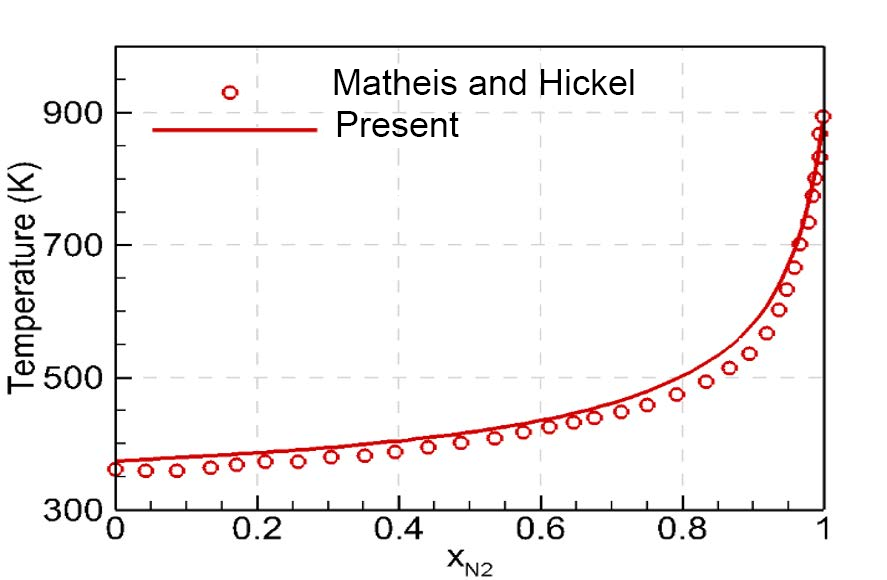
\includegraphics[width=0.50\linewidth]{mixing_temperature_C12_N2.png}
        \end{center}
        \caption{Comparison of predicted equilibrium mixing temperatures $T_{eq}$ for n-dodecane/nitrogen mixtures between Matheis and Hickel~\cite{matheis2018multi} and the current model.}
        \label{v6}
    \end{figure}

    \subsection{Validation and verification of the CFD solver} \label{App:vali:CFD}
    Two 1D shock tube simulations are conducted to validate and verify the CFD solver. First, Sod shock tube~\cite{sod1978survey} is used to test the CFD solver with the ideal gas model, and the results are shown in Fig.~\ref{vali1ST}. The pressure and temperature evolution show a good agreement with the exact solution. Although the PIMPLE algorithm is pressure-based, the 1D Sod shock tube results clearly show that this compressible version of PIMPLE algorithm can well capture the shock wave and accurately predict compressible flows. Moreover, the results show that the scheme is not dissipative, as the sharp gradients (e.g., near the shock) are accurately captured with only 200 grid cells and there is no spurious oscillation near the high gradients. Second, results from a shock tube simulation with phase change are compared with Chiapolino et al.'s simulation results~\cite{chiapolino2017simple}, as shown in Fig.~\ref{vali2ST}. The shock tube is filled with a homogeneous water-air mixture, and the initial discontinuity is located at 0.5 m. Chiapolino et al.'s model used the Noble Abel Stiffened Gas (NASG) EOS and also assumed mechanical and thermodynamic equilibrium. Therefore, their results can also capture the phase change in the shock tube, which is valuable as a reference to verify the implementation of the VLE-based CFD simulation framework in this study both qualitatively and quantitatively. Good agreements were obtained in terms of the evolution of pressure and temperature at the contact discontinuity.
    Note that Chiapolino et al. used a fully compressible CFD solver (based on MUSCL Hancock method using van Leer’s slope limiter and HLLC Riemann solver), while the CFD solver in this study uses a pressure-based PIMPLE method (which can be called a ``low-Mach'' solver but was extended to a transonic version). For this reason, the fact that both CFD solvers agree with each other can imply that the observed discrepancy between the CFD results with and without phase change (i.e., with and without VLE) in Fig.~\ref{v9} should not come from numerical implementation but should come from the real physics of the shock tube problem.
    \begin{figure}[htbp]

            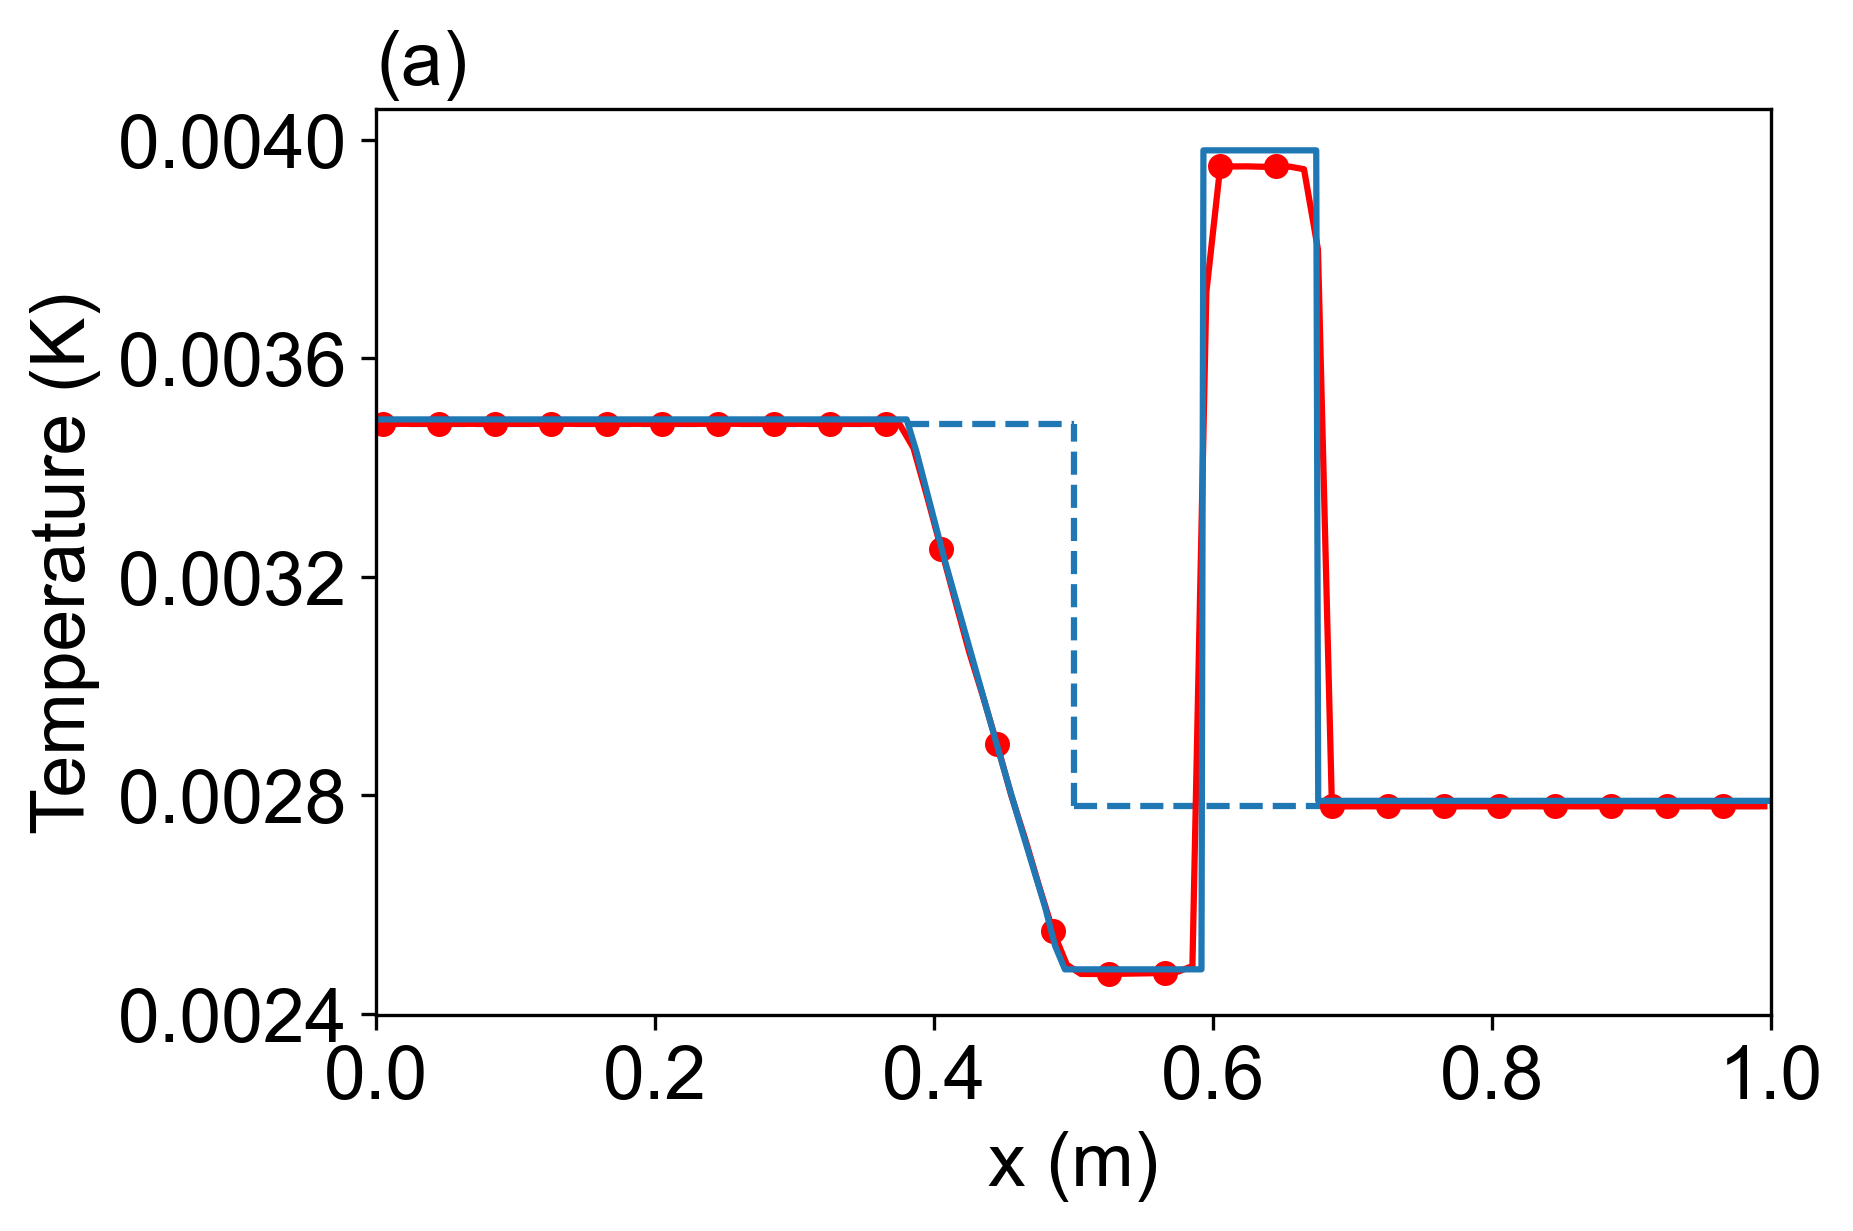
\includegraphics[width=0.465\linewidth]{sodT_v2.png}
            \includegraphics[width=0.435\linewidth]{sodP_V2.png}

        \caption{Validation of the VLE-based CFD solver by Sod shock tube simulations. Initial conditions: $P_{\rm{left}} = 1$ Pa, $P_{\rm{right}} = 0.1$ Pa, $T_{\rm{left}} = 0.00348$ K, $T_{\rm{right}} = 0.00278$ K, the initial discontinuity is at $x=0.5$ m; fluid: air; $t=0.1$ s; 200 grid cells, CFL = 0.2.}
        \label{vali1ST}
    \end{figure}
    
    
     \begin{figure}[htbp]

        \centering

            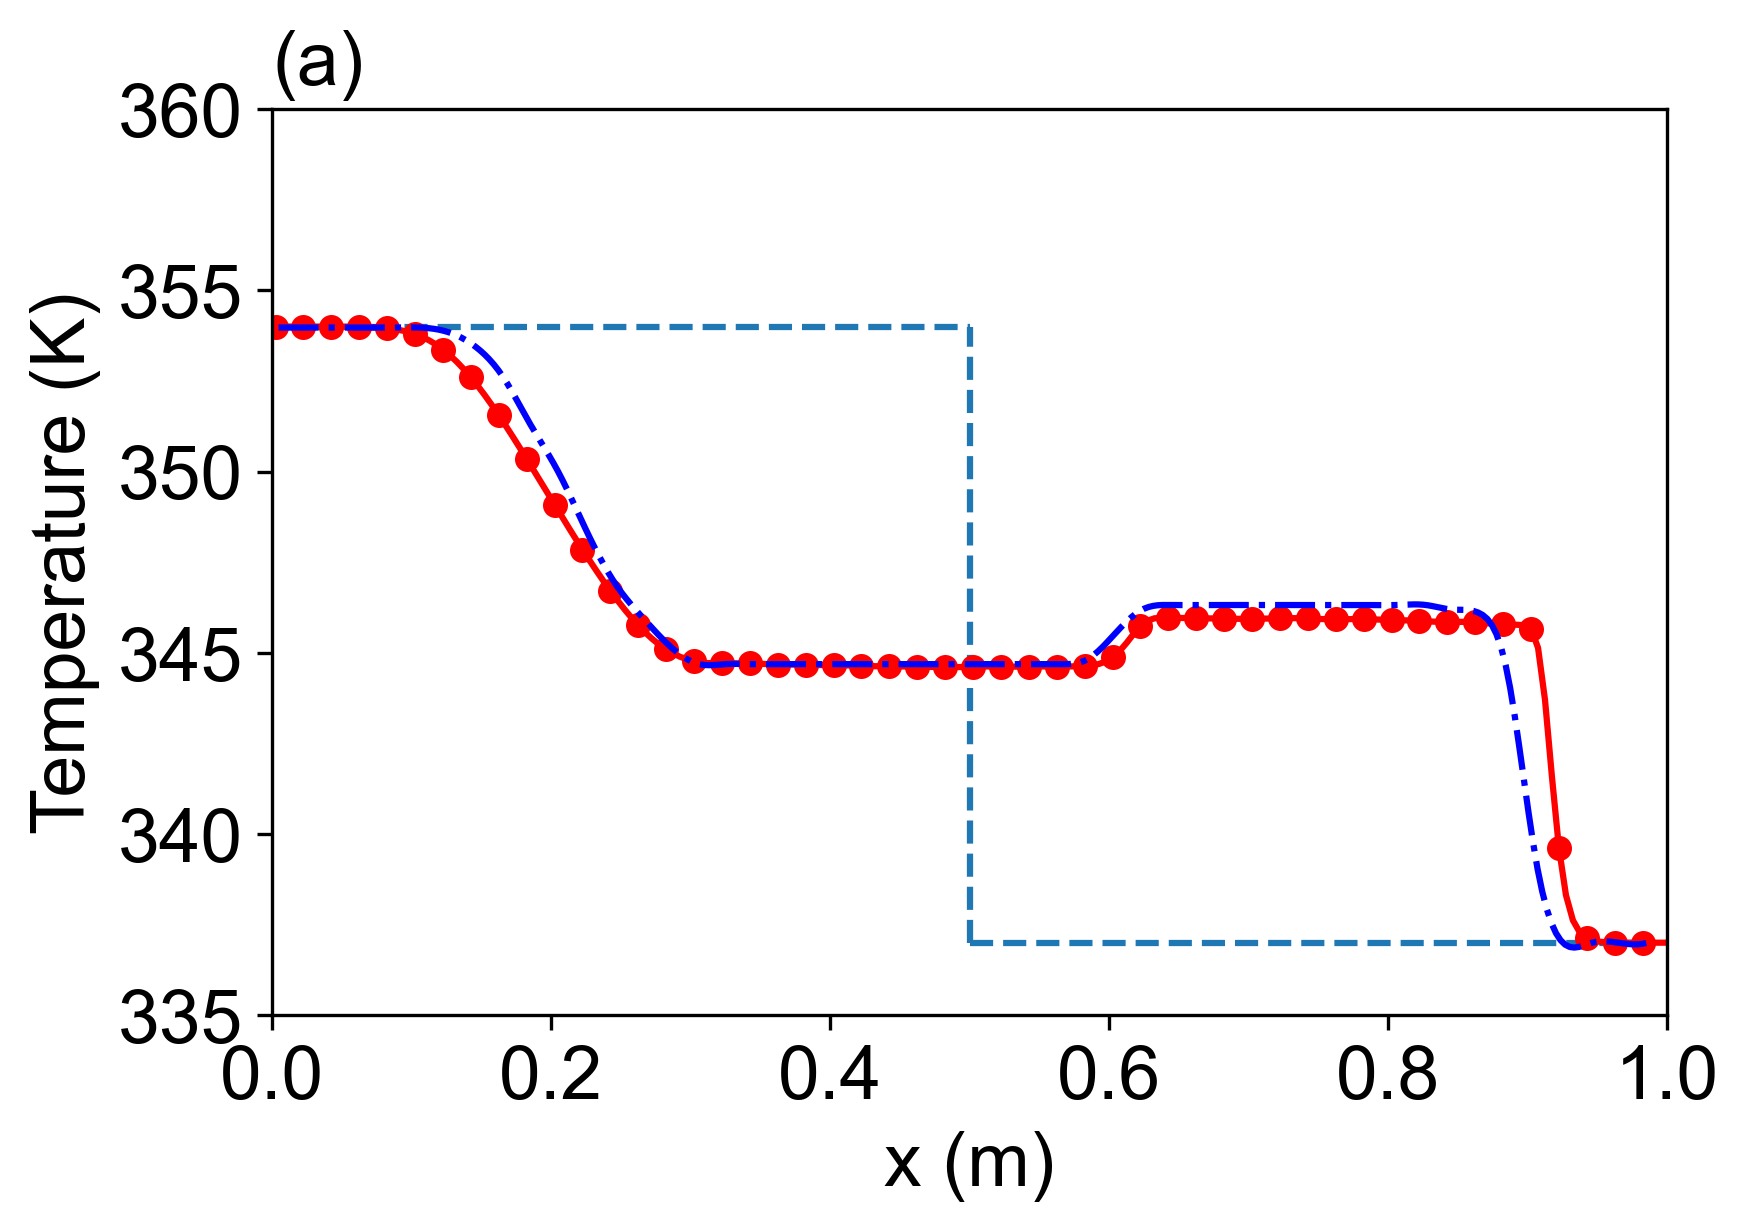
\includegraphics[width=0.45\linewidth]{valiT_v2.png}
            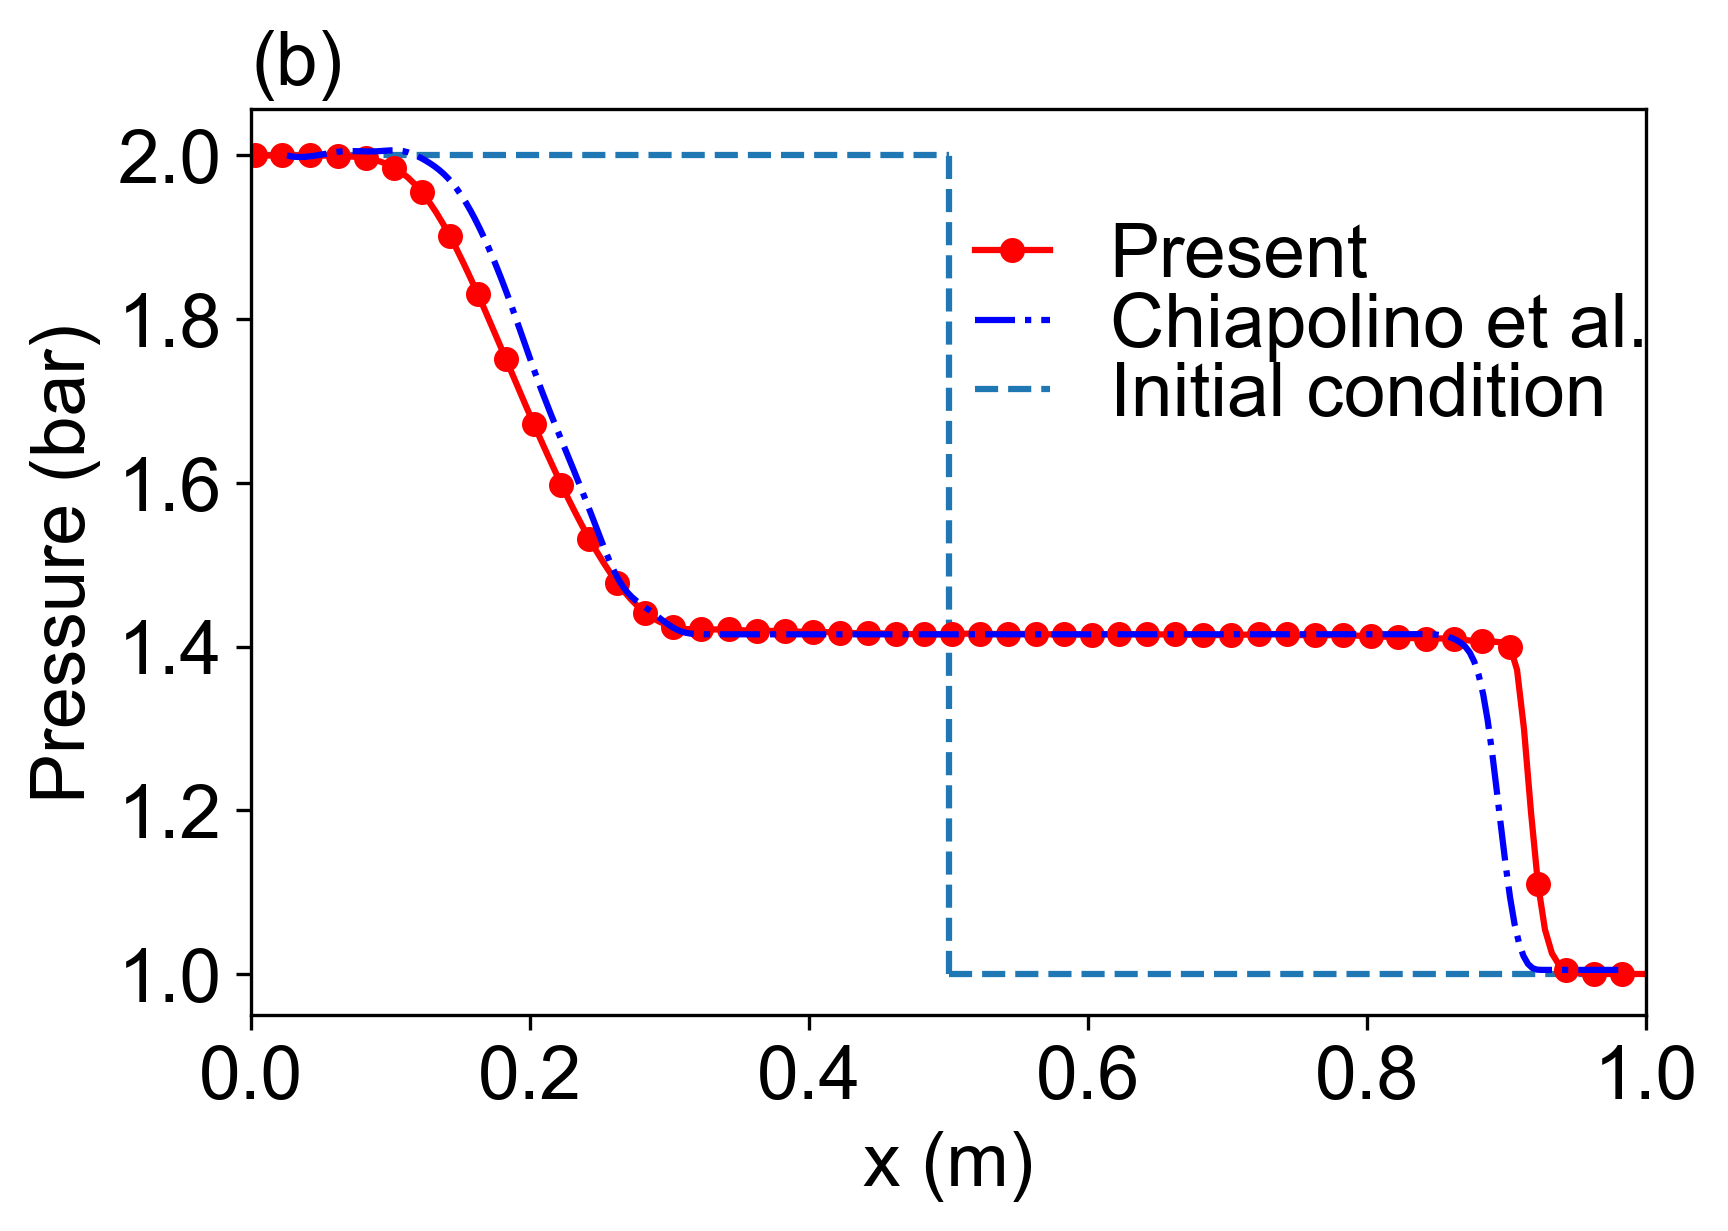
\includegraphics[width=0.45\linewidth]{valiP_v2.png}
        \caption{Verification of the VLE-based CFD solver by Chiapolino et al.'s shock tube simulations ~\cite{chiapolino2017simple}. Initial condition: $P_{\rm{left}} = 2$ bar, $P_{\rm{right}} = 1$ bar, $T_{\rm{left}} = 354$ K, $T_{\rm{right}} = 337$ K, $Y_{\rm{H_2O,\ left}} = Y_{\rm{H_2O,\ left}} = 0.3$, $Y_{\rm{Air,\ left}} = Y_{\rm{Air,\ left}} = 0.7$; $t = 1.0$ ms, 200 grid cells, CFL = 0.1, the initial discontinuity is at $x=0.5$ m.}
        \label{vali2ST}
    \end{figure}

    LES of a jet-in-crossflow is also conducted to validate the CFD solver. The results are compared with Su and Mungal's experimental data \cite{su2004simultaneous}. The experiments were performed in an updraft wind tunnel with air as the crossflow fluid and nitrogen as the jet fluid. The crossflow and nitrogen are both at 300 K and 1 atm. Nitrogen is seeded with acetone vapor to 10\% by volume for diagnostic purposes, which is also considered in the simulation. The tunnel crossflow velocity profile has a peak value of $v_{\infty}=2.95\ \rm{m/s}$. Nitrogen is injected from a nozzle with inner diameter $d=4.53\ \rm{mm}$, the jet average velocity is $u_0=16.9\ \rm{m/s}$. The mesh in the simulation contains 1.3M cells in total, and the average cell size is 2.3 mm. A finer mesh ($500\ \rm{\mu m}$) is used to capture the detailed flow structure near the injection nozzle. Based on the binary diffusivity of acetone and air ($D=0.104\ \rm{cm}^2\rm{s}^{-1}$) and the kinematic viscosity of air ($\nu=0.155\ \rm{cm}^2\rm{s}^{-1}$), Schmidt number, $Sc\equiv \nu/D$, of the system is 1.49. In Fig.~\ref{valiJIC}, the center streamline and \ce{N2} centerline of time-averaged field are compared between the simulation and experiments. The center streamline is the streamline that goes through the center of injector, and the \ce{N2} centerline is the line of maximum \ce{N2} concentration points at fixed-y planes. Length scales are properly normalized by the factor $rd$, where $d$ is the jet diameter (4.53 mm), $r$ is ratio of jet velocity to crossflow velocity: $r\equiv u_0/v_{\infty}=5.7$. The simulation results agree well with the experimental data at $x>2rd$, but show a small deviation near the injection nozzle.
    This validation indicates that our CFD solver and LES models can accurately predict the mixing process at least for ideal gas.

    \begin{figure}[htb]
        \begin{center}
            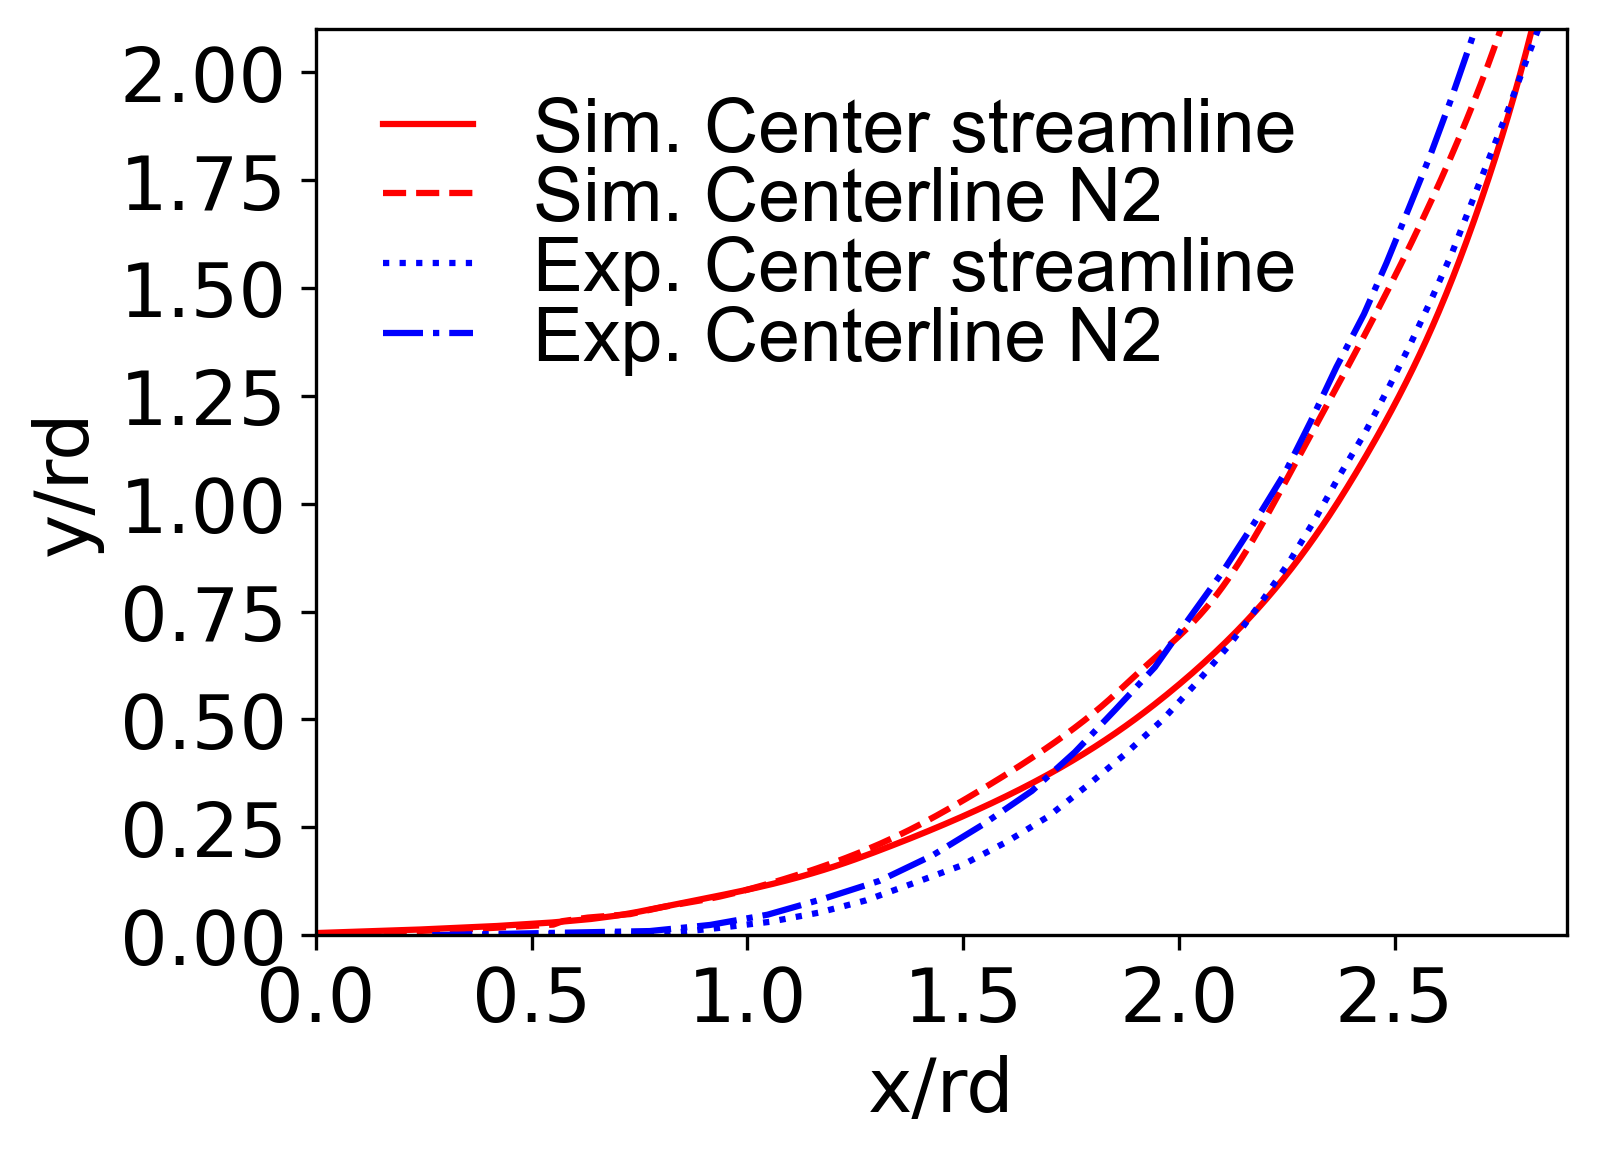
\includegraphics[width=0.5\linewidth]{valiJIC.png}
        \end{center}
        \caption{Comparison of a jet-in-crossflow between the present model prediction and experimental data~\cite{su2004simultaneous}. Blue: experimental data; red: simulation prediction.}
        \label{valiJIC}
    \end{figure}









%%%%%%%%%%%%%%%%%%%%%%%%%%%%%%%%%%%%%%%%%%%%%%%%%%%%%%%%%%%%%%%%%%%%%%%%%%%%%%%%
